\documentclass[
	openany,
	% -- opções da classe memoir --
	12pt,				% tamanho da fonte
   % openright,
	%twoside,
    oneside,
    % para impressão em verso e anverso. Oposto a oneside
	a4paper,			% tamanho do papel. 
	brazil				% o último idioma é o principal do documento
	]{abntex2}

% ---
% Pacotes básicos 
% ---

\usepackage{fontspec}
\setmainfont{Arial}

\usepackage[utf8]{inputenc}		% Codificacao do documento (conversão automática dos acentos)
\usepackage{indentfirst}		% Indenta o primeiro parágrafo de cada seção.
\usepackage{color}				% Controle das cores
\usepackage{graphicx}			% Inclusão de gráficos
\usepackage{microtype} 			% para melhorias de justificação
\usepackage{multicol}			% multiplas colunas no texto
\usepackage{subcaption}
\usepackage{caption}
\usepackage{float}
\usepackage{amsmath}
\usepackage{amssymb}
\usepackage{amsthm}
\usepackage{lipsum}
\usepackage{blindtext}


% ---
% ---
% Pacotes de citações
% ---
\usepackage[brazilian]{backref}	 % Paginas com as citações na bibl
\usepackage[alf]{abntex2cite}	% Citações padrão ABNT

% --- 
% CONFIGURAÇÕES DE PACOTES
% --- 

% ---
% Configurações do pacote backref
% Usado sem a opção hyperpageref de backref
\renewcommand{\backrefpagesname}{Citado na(s) página(s):~}
% Texto padrão antes do número das páginas
\renewcommand{\backref}{}
% Define os textos da citação
\renewcommand*{\backrefalt}[4]{
	\ifcase #1 %
		Nenhuma citação no texto.%
	\or
		Citado na página #2.%
	\else
		Citado #1 vezes nas páginas #2.%
	\fi}%
% ---

% ---
% Informações de dados para CAPA e FOLHA DE ROSTO
% ---
\titulo{Aplicativo móvel de apoio à gestão de eventos acadêmicos}
\autor{Luidi Matheus Silva de Oliveira\\Luiz Fellipe Saidler Leitier}
\local{Campos dos Goytacazes}
\data{2021}
\orientador{Ronaldo Amaral Santos}
\coorientador{}


\instituicao{%
	Instituto Federal Fluminense campus Campos Centro
    \par
  	Curso de Bacharelado em Sistemas de Informação
}

\tipotrabalho{Trabalho de Conclusão de Curso}
% O preambulo deve conter o tipo do trabalho, o objetivo, 
% o nome da instituição e a área de concentração 
\preambulo{Monografia apresentada ao Curso de Bacharelado em Sistemas de Informação do Instituto Federal Fluminense campus Campos Centro, como requisito parcial para obtenção do título de Bacharel em Sistemas de Informação.}
% ---


% ---
% Configurações de aparência do PDF final

% alterando o aspecto da cor azul
\definecolor{blue}{RGB}{41,5,195}

% informações do PDF
\makeatletter
\hypersetup{
     	%pagebackref=true,
		pdftitle={\@title}, 
		pdfauthor={\@author},
    	pdfsubject={\imprimirpreambulo},
	    pdfcreator={LaTeX with abnTeX2},
		colorlinks=true,       		% false: boxed links; true: colored links
    	linkcolor=blue,          	% color of internal links
    	citecolor=blue,        		% color of links to bibliography
    	filecolor=magenta,      		% color of file links
		urlcolor=blue,
		bookmarksdepth=4
}
\makeatother
% --- 

% --- 
% Espaçamentos entre linhas e parágrafos 
% --- 

% O tamanho do parágrafo é dado por:
\setlength{\parindent}{1.3cm}

% Controle do espaçamento entre um parágrafo e outro:
\setlength{\parskip}{0.2cm}  % tente também \onelineskip

% ---
% compila o indice
% ---
\makeindex
% ---

% ----
% Início do documento
% ----
\begin{document}

% Seleciona o idioma do documento (conforme pacotes do babel)
%\selectlanguage{english}
\selectlanguage{brazil}

% Retira espaço extra obsoleto entre as frases.
\frenchspacing 

% ----------------------------------------------------------
% ELEMENTOS PRÉ-TEXTUAIS
% ----------------------------------------------------------
% \pretextual
%\begin{figure}[h]
%\centering % este comando é usado para centralizar a figura
%\includegraphics[width=7cm]{figuras/logo_ufrpe_horizontal.png}\\
%\end{figure}

% \begin{figure}[ht]
% \centering
% \begin{minipage}[b]{0.45\textwidth}
% \includegraphics[height=3cm]{figuras/logo_ufrpe_horizontal.png}
% \end{minipage}
% \qquad
% \begin{minipage}[b]{0.45\textwidth}
% \includegraphics[height=2.5cm]{figuras/logo_bsi.pdf}
% \end{minipage}
% \end{figure}

%\begin{minipage}[t]{1\textwidth}
% 	\begin{figure}[ht]
% 		\includegraphics[height=3cm]{figuras/logo_ufrpe_horizontal.png}
% 		\hspace{4.5cm}
%     	\includegraphics[height=2.5cm]{figuras/logo_bsi.pdf}
% 	\end{figure}    
%\end{minipage}

% ---
% Capa
% ---
\imprimircapa
% ---
% ---
% Folha de rosto
% (o * indica que haverá a ficha bibliográfica)
% ---
\imprimirfolhaderosto
% % ---

% % dedicatoria
% \begin{dedicatoria}
   \vspace*{\fill}
   \centering
   \noindent
   \textit{À \ldots\\} \vspace*{\fill}
\end{dedicatoria}

% % agradecimentos
% \begin{agradecimentos}
Agradeço à \ldots

\end{agradecimentos}

% % epigrafe
% \begin{epigrafe}
    \vspace*{\fill}
	\begin{flushright}
		\textit{``A persistência é o caminho do êxito.'' \\
		(Charles Chaplin)}
	\end{flushright}
\end{epigrafe}

% % resumo e abstract
% \setlength{\absparsep}{18pt} % ajusta o espaçamento dos parágrafos do resumo
\begin{resumo}
 
\lipsum[1]

 \textbf{Palavras-chave}: palavra 1, palavra 2, \ldots.
\end{resumo}


% \begin{resumo}[Abstract]
 \begin{otherlanguage*}{english}
  
  \lipsum[1] 

   \vspace{\onelineskip}
 
   \noindent 
   \textbf{Keywords}:  word 1, word 2, \ldots.
 \end{otherlanguage*}
\end{resumo}

% ---
% inserir lista de ilustrações
% ---
\pdfbookmark[0]{\listfigurename}{lof}
\listoffigures
\cleardoublepage
% ---

% % ---
% % inserir lista de tabelas
% % ---
% \pdfbookmark[0]{\listtablename}{lot}
% \listoftables*
% \cleardoublepage
% % ---

% ---
% inserir lista de abreviaturas e siglas
% ---
\begin{siglas}
  \item[IFF] Instituto Federal Fluminense
  \item[JSON] \textit{JavaScript Object Notation}
  \item[IHC] Interação Humano–Computador
  \item[MVP] \textit{Minimum Viable Product}
  \item[API] \textit{Application Programming Interface}
  \item[PHP] \textit{PHP: Hypertext Preprocessor}
  \item[HTTP] \textit{Hypertext Transfer Protocol}
  \item[SQL] \textit{Structured Query Language}
  \item[CPF] Cadastro de Pessoas Físicas
  \item[CSV] \textit{Comma-Separated Values}
\end{siglas}
% ---

% % ---
% % inserir o sumario
% % ---
\pdfbookmark[0]{\contentsname}{toc}
\tableofcontents*
\cleardoublepage
% ---



% ----------------------------------------------------------
% ELEMENTOS TEXTUAIS
% ----------------------------------------------------------
\textual

% ----------------------------------------------------------
% inclusao das secoes do texto
% ----------------------------------------------------------
\chapter{Introdução}

Com o crescente avanço da formação acadêmica e das universidades, os eventos acadêmicos tornam-se cada vez mais frequentes. Esses eventos são de grande importância para a formação, visto que é uma forma do aluno interagir com profissionais da área, além de poder submeter artigos acadêmicos sendo fundamentais para a comunidade científica, agregando mais experiência e conhecimento para a formação do aluno.

Em geral, os eventos acadêmicos são compostos por atividades como: congressos, seminários, cursos, mesas-redondas, entre outros, gerando assim grande fluxo de alunos durante essas atividades, e devido à maioria gerar certificados de participação, a presença do aluno deve ser registrada. Com isso, o gerenciamento do evento sem um software ou aplicação resulta em um evento com mais riscos e gargalos. 

Atualmente, há diversas ferramentas digitais para controle de eventos em geral. Umas delas são as redes sociais, como \textit{Facebook} e \textit{Instagram}, que facilitam a divulgação e comunicação com o público alvo, porém são superficiais quando o assunto é gestão. Contudo, algumas plataformas \textit{web} e móveis foram criadas com esse tipo de finalidade, e oferecem funcionalidades para administração de eventos, como \textit{Doity} e \textit{Eventbrite}. 
Conforme a aumento da demanda de eventos acadêmicos, o IFF se viu necessitado de uma plataforma para centralizar a administração deles, sendo assim foi desenvolvido o \textit{website} Eventos IFF.

\section{Objetivos}
\subsection{Objetivos Gerais}

Desenvolver um protótipo interativo da solução para o gerenciamento de eventos integrada a plataforma \textit{web} IFF Eventos e desenhar a arquitetura de um sistema para gestão de eventos.

\subsection{Objetivos Específicos}

Dentre os objetivos específicos do trabalho de conclusão, destacam-se:
\begin{itemize}
    \item Validação da funcionalidade em cenário real de evento acadêmico;
    \item Analisar o cenário de utilização desse tipo de aplicativo, observando e analisando os requisitos necessários para atender a demanda;
    \item Utilizar técnicas de prototipagem para construir um protótipo interativo e próximo da solução proposta;
    \item Construir diagramas para definição da arquitetura da solução. 
\end{itemize}

\section{Justificativa}

Apesar da existência de aplicações para gestão de eventos, as mesmas têm suas principais funcionalidades monetizadas, tornando custosas suas utilizações. Dessa forma, visando contribuir com o IFF, foi decidido realizar o desenvolvimento de um projeto para uma aplicação focada no gerenciamento de eventos acadêmicos utilizando tecnologia móvel e baseando-se na estrutura de organização da plataforma web Eventos IFF.

Com base nisto espera-se que por meio desta aplicação a gestão dos eventos seja otimizada, minimizando assim os riscos e gargalos e impactando positivamente a comunidade acadêmica.

\section{Organização da monografia}

O conteúdo deste trabalho está dividido em 4 capítulos. No Capítulo 2 é apresentado  uma revisão bibliográfica sobre \textit{Firebase} e o conceito de prototipação. No Capítulo 3 é apresentado a metodologia... [vai ser completado futuramente]. Por fim, no Capítulo 4 é apresentado... [vai ser completado futuramente].

\chapter{Revisão Bibliográfica}

\section{Firebase}

\textit{Firebase} é um produto da \textit{Google} que engloba serviços para realização de  processos internos para algumas plataformas e linguagens de programação. Para aplicações que necessitam, por exemplo, de respostas rápidas para um dado modificado ou acrescentado na base dados, o Firebase se torna ideal para realização desse tipo de serviço \cite{firebase}.

O Firebase é dividido em alguns tipos de serviços, que estão listados e detalhados a seguir.

\begin{itemize}
    \item \textit{Real-time Database}: Serviço de armazenamento em nuvem, onde os dados são armazenados e estruturados em formato \textit{JavaScript Object Notation} (JSON). Cada cliente é associado aos seus dados e automaticamente são sincronizados, realizando uma resposta rápida quando algum dado é atualizado \cite{firebase};
    \item \textit{Authentication}: Gerencia as requisições referentes a autenticação, tais como \textit{login}. Permite que o usuário crie perfis de autenticação usando \textit{e-mail} e senha, número de telefone, entre outros \cite{firebase};
    \item \textit{Storage}: Armazena conteúdo gerado pelos clientes, tais como arquivos de mídia, e realiza uma transferência segura desse conteúdo quando solicitado \cite{firebase}. 
\end{itemize}

\section{Prototipação}

No processo de desenvolvimento de um sistema, é fundamental a realização de testes antes da versão ser finalizada. Quase sempre os requisitos definidos no início do projeto não atendem completamente ao usuário final, e uma mudança no \textit{software} após sua finalização pode ser muito custoso \cite{prototipacao}.

O ato da prototipação auxilia a enxergar os requisitos que precisam ser revisados ou até retirados do projeto. A prototipação em um projeto de desenvolvimento é uma ótima forma de comunicação entre o usuário alvo e desenvolvedor, pois provê um \textit{feedback} mais realista sobre o contexto onde o \textit{software} pretende ser utilizado \cite{prototipacao}.

A prototipação em Interação Humano–Computador (IHC) conta com algumas técnicas para a sua execução. Para o desenvolvimento deste trabalho, foi decidido desenvolver um protótipo que oferecesse interatividade, aumentando assim a experiência e imersão durante sua utilização.

\subsection{Figma}

\textit{Figma} é uma ferramenta de \textit{design} colaborativa em nuvem, lançada em 2016, e com funcionamento em navegador, sendo possível utilizar em qualquer sistema operacional que execute um navegador da \textit{web} \cite{nguyen}. Por oferecer uma plataforma colaborativa e em nuvem, o \textit{Figma} permite que desenvolvedores, que estejam distantes geograficamente, possam estar atuando e colaborando no mesmo projeto de prototipação \cite{nascimento}.

Existem outras soluções para prototipação no mercado similares ao \textit{Figma}, como o \textit{Adobe XD}. No entanto, o \textit{Figma} apresenta algumas vantagens que o faz ser escolhido para projetos de prototipação \cite{teplov}. Algumas dessas vantagens são:

\begin{itemize}
    \item Por ser uma aplicação baseada na \textit{web}, é possível de ser executada em mais sistemas operacionais. \textit{Adobe XD} apenas pode ser executado em sistema operacional \textit{Windows} e \textit{Mac} \cite{teplov};
    \item É possível compartilhar mais projetos com a conta grátis. \textit{Adobe XD} permite apenas um projeto compartilhado \cite{teplov}.
\end{itemize}
\chapter{Análise do Problema}

Este capítulo tem como objetivo fazer uma análise e contextualização dos problemas descritos por esse trabalho. Na seção 3.1 é abordado sobre o conceito de evento acadêmico e seus desafios atuais. Na seção 3.2 é descrito e comparado algumas soluções presentes no mercado para gestão de eventos. Na seção 3.3 é apresentada a solução proposta por esse trabalho para auxílio na gestão de eventos da plataforma Eventos IFF. Por fim, na seção 3.4 é apresentado diagramas descrevendo o cenário do ciclo de vida dos eventos na plataforma Eventos IFF.

\section{Gestão de eventos acadêmicos}

Os eventos científicos ou acadêmicos são eventos onde ocorrem encontros entre profissionais, cientistas, especialistas e estudantes para compartilhar e obter conhecimentos sobre uma determinada área de interesse. Esses encontros promovem oportunidades para troca de experiência e atualizações sobre a área através de divulgação de novos conhecimentos \cite{lacerda}. Deste modo, os eventos acadêmicos se tornam importantes para a formação acadêmica do aluno, pois podem proporcionar diversos conhecimentos importantes para sua atuação na área.

Esses eventos podem ser compostos por diversas atividades, como: congressos, convenções, \textit{workshops}, fóruns, painéis, entre outras atividades. Além disso, em geral, os eventos acadêmicos possuem uma comissão organizadora \cite{araujo}.

Com o passar dos anos, os eventos acadêmicos passaram a ter maior visibilidade através do uso da internet, visto que antes dessa evolução, esses eventos eram apenas reconhecidos nos ambientes acadêmicos institucionalizados nas universidades \cite{araujo}. Mediante o exposto, os organizadores desses eventos passam por desafios em conseguir administrar os dados gerados antes, durante e depois do evento. Esses dados consistem, por exemplo, no registro da presença de um aluno em determinada atividade, o que é de extrema importância para a gerar o certificado de participação do aluno.

\section{Soluções no mercado}

No mercado existem algumas plataformas e aplicativos móveis que trazem soluções para gestão de eventos, cada um atendendo a critérios como: divulgação, administração de participantes, registro de presença, entre outras funcionalidades. A seguir é listada algumas das soluções mais conhecidas e utilizadas no mercado para critério de comparação e análise deste trabalho.

\subsection{Doity}

Doity é uma plataforma que oferece várias funções para gerenciamento de eventos, ou seja, desde a etapa de divulgação até a emissão de certificados. Em seu \textit{site} é informado que a Doity foi utilizada em mais 100 mil eventos presentes em mais de 1500 cidades. 

A plataforma permite realizar eventos onde a inscrição é gratuita, sem realizar nenhum tipo de cobrança pelo uso da ferramenta. A cobrança é feita quando o evento realiza inscrições pagas, onde é cobrado 10\% do valor da inscrição como taxa.

No \textit{site} da plataforma é destacada as principais soluções que a Doity proporciona. Abaixo é listado essas funcionalidades:

\begin{itemize}
    \item \textit{Site} do evento: é possível realizar a criação de uma página \textit{web} com as ferramentas da plataforma, onde o usuário consegue customizar o conteúdo, como textos, imagens e \textit{design}.
    \item Inscrições: o usuário pode realizar a inscrição no evento. Eventos onde tenha algum valor na inscrição, ele pode estar realizando o pagamento via cartão de crédito ou boleto bancário pelo \textit{site}.
    \item Credenciamento: pela plataforma é possível gerar crachás customizáveis para distribuir para os participantes. Através do crachá é possível realizar o credenciamento através do aplicativo móvel. O credenciamento envolve realizar registro de entrada e saída do participante na atividade.
    \item Inscrições em atividades: o participante pode se inscrever em cada atividade separadamente. Com isso, pela interface de gerenciamento, o organizador poderá ter um controle maior sobre as vagas nas determinadas atividades.
    \item Certificados: o organizador pode emitir certificados customizáveis pela plataforma e enviar por e-mail para os participantes, além de poder imprimir. Os certificados emitidos recebem um código de validação, que podem ser usados na plataforma da Doity para verificar a veracidade do certificado.
    \item Trabalhos científicos: a Doity oferece uma área onde o organizador pode criar um formulário customizável para envio de trabalhos científicos. Além disso, ele pode definir a forma que o trabalho poderá ser avaliado, como os critérios de avaliação e o modo de visualização das notas.
\end{itemize}

No \textit{site} da Doity contém uma área onde é possível procurar eventos cadastrados na plataforma, podendo filtrar por área, Estado, período do dia e modalidade do evento. Essa funcionalidade contribui na divulgação e procura de eventos.

Quanto à quantidade de participantes que um evento pode ter inscrito pela plataforma da Doity, para eventos onde tem valor de cobrança na inscrição, a quantidade de participantes é ilimitada. No entanto, para eventos com inscrição gratuita, existe um limite de até 3000 participantes. 

\subsection{Sympla}

A Sympla também oferece soluções para cada etapa da jornada do evento. No seu painel de controle, a plataforma conta com uma interface gráfica com várias informações em tempo real para auxiliar o organizador durante o evento, o que se torna um diferencial.

Em seu \textit{site}, a Sympla informa que foram mais de 600 mil eventos realizados utilizando a ferramenta em mais de 2500 cidades diferentes. Quanto ao custo, para eventos com inscrições gratuitas, não é cobrado algum valor, e o organizador do evento tem acesso a todas as funcionalidades da plataforma. Para eventos com valor na inscrição, a Sympla cobra 10% do valor do ingresso como taxa.

Abaixo é listado as principais funcionalidades destacadas pela Sympla:

\begin{itemize}
    \item \textit{Hotsite} para eventos: é possível criar uma simples página \textit{web} para a divulgação do evento, com ferramentas que tornam a página personalizável e responsiva.
    \item Compartilhamento de níveis de acesso: o organizador do evento pode conceder acesso para outros usuários também terem acesso ao painel administrativo da Sympla, assim dividindo a organização do evento com outros usuários. O acesso pode ser concedido com nível de acesso. Cada nível de acesso permite usar determinadas funcionalidades administrativas.
    \item Impressão de crachás para eventos: a plataforma oferece uma simples customização do conteúdo principal do crachá, podendo informar qual dado principal do participante aparecerá no crachá.
    \item \textit{Check-in}: o organizador pode realizar o credenciamento do participante por algumas formas usando a Sympla, como utilizar o aplicativo móvel para realizar a leitura de \textit{QRCode} de identificação do participante; assinalar diretamente a participação na plataforma; usar um leitor de código de barras para ler o código de barras do crachá; ou, para situações sem conexão com a internet, é possível gerar uma planilha em Excel, registrar as presenças e após isso importar no \textit{site} a planilha quando estiver com conexão com a internet novamente.
    \item Certificados de participação: é possível gerar certificados de participação e enviar para os participantes. A plataforma permite customizar o certificado.
\end{itemize}

Através do \textit{site} da Sympla é possível encontrar os eventos cadastrados na plataforma, podendo filtrar por local e categorias, por exemplo. Não foi encontrado em suas funcionalidades a possibilidade de cadastrar atividades dentro do evento, o que impossibilita registrar presença e gerar certificado por atividade, apenas de todo o evento.

\subsection{Eventbrite}

\textit{Eventbrite} oferece serviço para gerenciamento de eventos para vários países. Em seu \textit{site}, é informado que a \textit{Eventbrite} foi usada em 3 milhões de eventos em mais de 170 países durante o ano de 2017.

Em eventos com inscrição gratuita, não é cobrada taxa sobre o uso da plataforma. A \textit{Eventbrite} divide o valor de sua taxa no ingresso do evento em 3 planos, os quais estão listados abaixo:

\begin{itemize}
    \item \textit{Essentials}: taxa de 6.99\% sobre o valor do ingresso. Oferece ferramentas básicas para gerenciar o evento, como venda de ingresso \textit{online} e aplicativo móvel para organizadores.
    \item \textit{Professional}: taxa de 9,99\% sobre o valor do ingresso. Traz as mesmas ferramentas do plano \textit{Essentials}, adicionando integração com venda de ingresso em \textit{site}, formulário de compra de ingresso personalizado e análise de venda detalhada.
    \item \textit{Premium}: a taxa de cobrança deste plano tem valor customizável, passando por avaliação da \textit{Eventbrite}. Nesse plano, o usuário tem todas as mesmas ferramentas do plano \textit{Professional}, adicionando aluguel de equipamentos e treinamento para o uso da ferramenta.
\end{itemize}

No \textit{site} da \textit{Eventbrite} é destacada as principais funcionalidades que a plataforma proporciona. Abaixo é listado essas funcionalidades:

\begin{itemize}
    \item Processamento de pagamento: a plataforma permite pagamento dos ingressos do evento de forma \textit{online}, fazendo o processamento e repasse desse valor.
    \item Aplicativo para organizador: é disponibilizado um aplicativo móvel para organizadores acompanharem vários aspectos do evento em tempo real.
    \item Página de evento: é possível realizar a criação de uma página \textit{web} do evento, com \textit{design} customizável, auxiliando na divulgação.
    \item Integração com redes sociais: a \textit{Eventbrite} possui integração com redes sociais como \textit{Facebook} e \textit{Instagram}, permitindo realização de algumas ações envolvendo essas redes sociais.
    \item \textit{Check-in}: é possível realizar o credenciamento por meio de leitura de \textit{QRCode} através do aplicativo móvel do organizador.
\end{itemize}

Em relação a criação de atividades dentro de um evento, não foi encontrada funcionalidade na Eventbrite que atenda a esse critério. Quanto a geração de certificados, em seu \textit{site} é mencionada a ferramenta \textit{EB Certs} da \textit{Eventbrite} para geração de certificados customizáveis. No entanto, desde 2020 essa ferramenta se encontra inativa para uso, o que deixa sem opção para geração de certificados pela plataforma.

\subsection{Facebook Eventos}

\textit{Facebook} Eventos é uma das funcionalidades da rede social \textit{Facebook}. Essa funcionalidade não tem como foco principal auxiliar no gerenciamento de eventos, apesar de possuir ferramentas para auxiliar um pouco nesse aspecto.

O uso dessa funcionalidade traz como grande benefício o seu alcance ao público, visto que pertence a uma das maiores redes sociais atuais. Com ela, é possível definir o local e período do evento, permitindo que usuários que utilizem o \textit{Facebook}, que sejam daquela região ou tenham amigos na rede social que interagem com esse evento, recebam a divulgação desse evento.

Para ampliar a divulgação do evento, o \textit{Facebook} permite utilizar sua ferramenta de criação de anúncios para divulgação de um evento. Com ela, é possível direcionar os anúncios para o público alvo do evento. Essa funcionalidade gera um custo através de um orçamento, onde varia para o tipo de configuração feita para o anúncio e tamanho do público alvo configurado.

Além disso, como coordenador do evento criado na plataforma, é possível ver quantas pessoas selecionaram a opção que tem interesse de participar do evento, o que traz uma dimensão da adesão que o evento está tendo com o público.

Porém, como dito anteriormente, o \textit{Facebook} Eventos não tem como foco principal oferecer funcionalidades para gerenciar eventos. Com isso, não é possível registrar presença e gerar certificados através da funcionalidade.

\section{Solução proposta}

Apesar das inúmeras ofertas dispostas no mercado, foi identificado que o desenvolvimento de um aplicativo seria uma hipótese, visto os requisitos e anseios da instituição, possibilitando também demais personalizações conforme as necessidades do requisitante.

Dentre todas as supracitadas, a que mais se aproximou do desejado foi o \textit{Doity}, porém não possui integração com sistemas terceiros, possibilitando apenas um botão no site, e há limitação de participantes em eventos grátis, características as quais são essenciais.

Para a escolha da plataforma, havia como requisito características indispensáveis. A mesma deveria ser gratuita, apresentasse uma fácil integração com a plataforma Eventos IFF, emissão de certificados e possibilidade de interação entre palestrante e inscritos, sendo assim optou-se pelo desenvolvimento de uma nova ferramenta.

\section{Diagramas da solução}

<colocar aqui diagramas de caso de uso e diagrama de classe conceitual>
\chapter{Metodologia}

Na Figura \ref{fig:metodologia} é ilustrado em fluxograma as etapas citadas neste capítulo para desenvolvimento do trabalho.

\begin{figure}[H]
    \centering
    \caption{Fluxograma das etapas executadas na metodologia}
    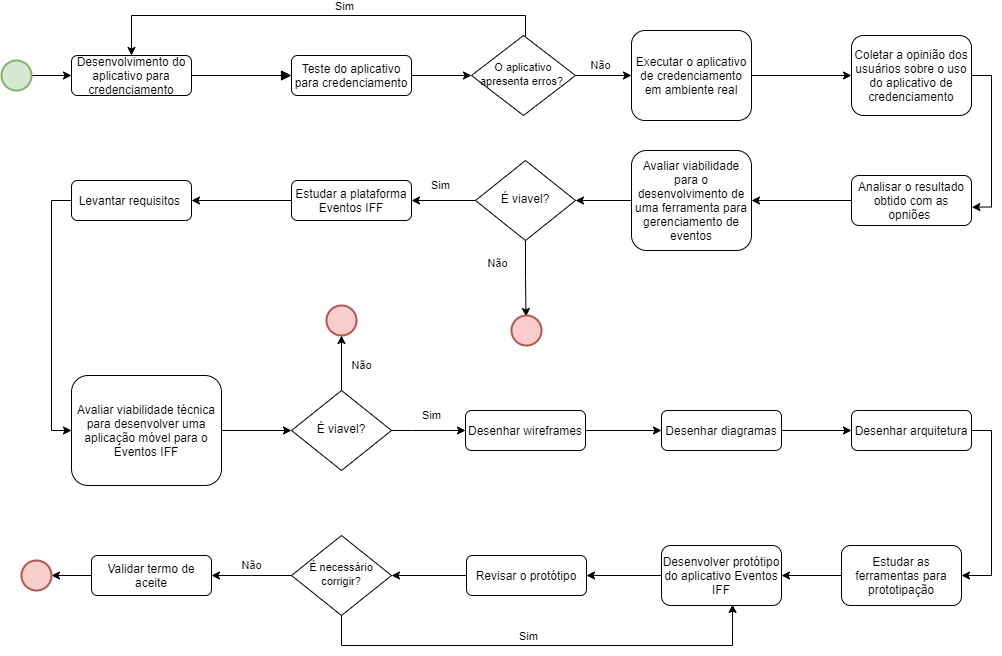
\includegraphics[scale=0.45]{figuras/metodologia.jpg}
    \label{fig:metodologia}
    \legend{Fonte: elaborado pelos autores}
\end{figure}

Esse trabalho foi desenvolvido seguindo as seguintes etapas, nas respectivas ordens: 

\begin{enumerate}
  \item Desenvolvimento de um aplicativo para validação da funcionalidade de credenciamento;
  \item Testes do aplicativo: nessa etapa é realizado testes executados pelos desenvolvedores para validação;
  \item Execução do aplicativo em ambiente real: o aplicativo é disponibilizado para uso no evento Congresso Integrado da Tecnologia da Informação (CITI) 2019;
  \item Coleta das opiniões dos usuários do aplicativo através de formulário;
  \item Análise do resultado obtido com o formulário de opinião;
  \item Avaliação da viabilidade da ferramenta para credenciamento em eventos acadêmicos;
  \item Estudo da plataforma \textit{web} Eventos IFF;
  \item Levantamento de requisitos para desenvolvimento do aplicativo móvel para o Eventos IFF;
  \item Avaliação da viabilidade técnica de implementação e integração de uma ferramenta móvel para a plataforma Eventos IFF;
  \item Desenho de \textit{wireframes} das funcionalidades levantadas com a análise de requisitos;
  \item Desenho dos diagramas de caso de uso e de classe;
  \item Desenho da arquitetura da solução;
  \item Estudo das ferramentas existentes para prototipação;
  \item Desenvolvimento do protótipo na plataforma selecionada;
  \item Revisão e correção do protótipo;
  \item Termo de aceite do protótipo.
\end{enumerate}
\chapter{Desenho da solução}

Esse capítulo tem como objetivo descrever como foi desenvolvido e desenhado a solução proposta por esse trabalho, além de apresentar resultados obtidos durante o processo.

\section{Solução proposta}

Como destacado por este trabalho anteriormente, há soluções dispostas no mercado que atendem a demanda de gestão de eventos. No entanto, foi identificado que o desenvolvimento de um aplicativo seria uma hipótese, visto os requisitos e anseios da instituição, possibilitando também demais personalizações conforme as necessidades do requisitante.

Dentre todas as citadas na Seção \ref{sec:mercado}, a que mais se aproximou do desejado foi o \textit{Doity}, porém não possui integração com sistemas terceiros, assim inviabilizando uma integração com a plataforma \textit{web} Eventos IFF. Além disso, há limitação na quantidade de participantes em eventos grátis, características as quais são essenciais.

Para a escolha da plataforma, havia como requisito características indispensáveis. A mesma deveria ser gratuita, deve apresentar uma fácil integração com a plataforma Eventos IFF, emissão de certificados e possibilidade de interação entre palestrante e inscritos, sendo assim optou-se pelo desenvolvimento de uma nova ferramenta.

\section{Diagramas da solução}

Na Figura \ref{fig:caso-de-uso} é ilustrado através do diagrama de uso as funcionalidades e ações que o usuário poderá executar no aplicativo Eventos IFF. O diagrama conta com dois atores. A audiência é o usuário que tem papel de participante do evento, já o organizador é o usuário que realiza a administração do evento, tendo acesso a todas as funcionalidades administrativas do aplicativo.

\begin{figure}[H]
    \centering
    \caption{Diagrama de caso de uso}
    \fbox{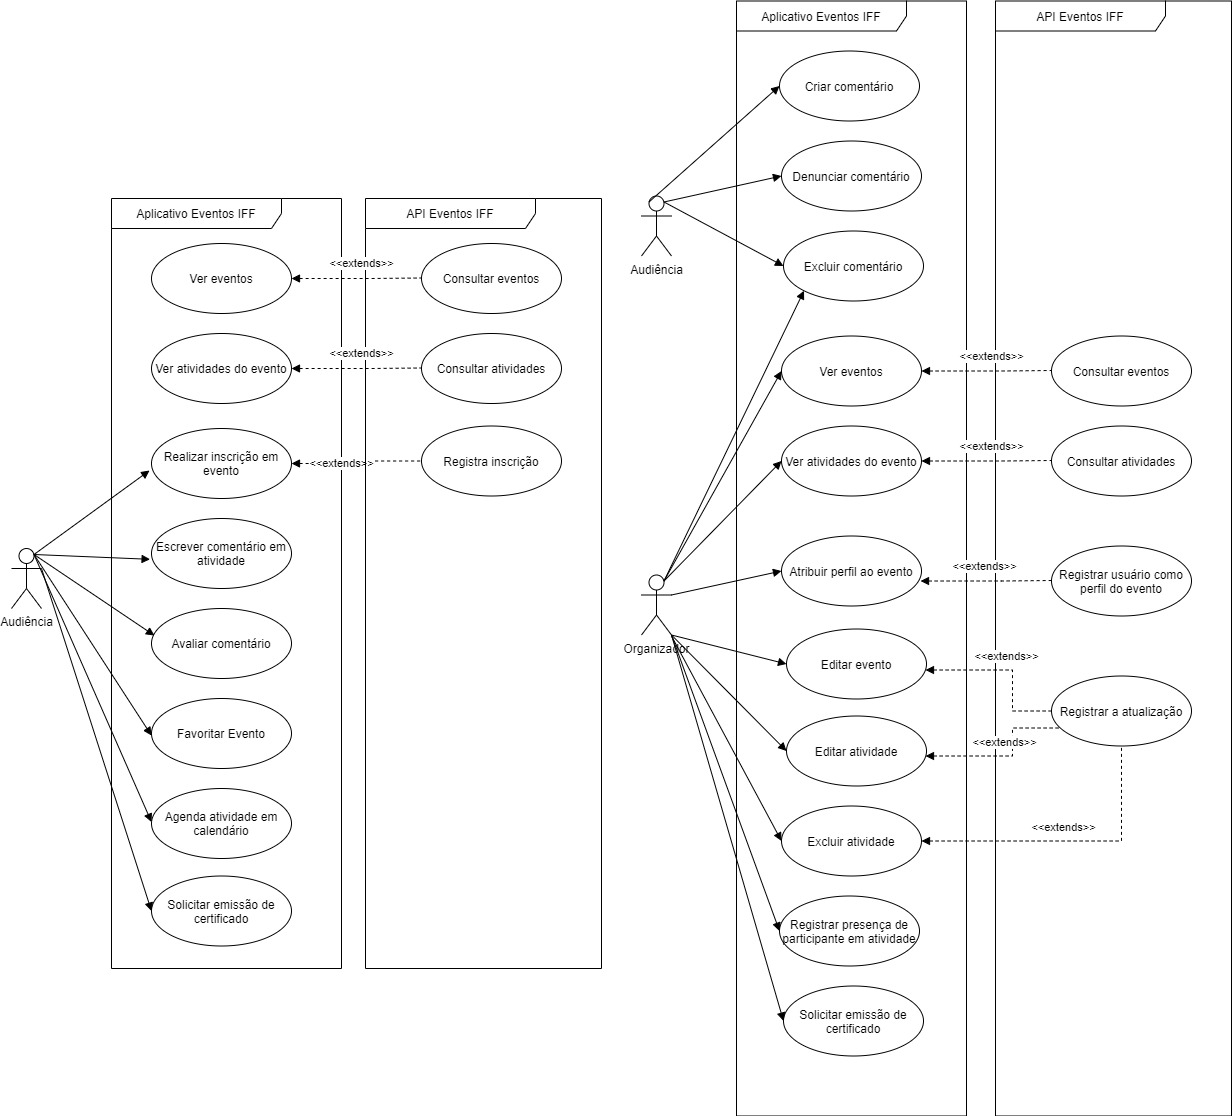
\includegraphics[scale=0.36]{figuras/caso-de-uso.jpg}}
    \label{fig:caso-de-uso}
    \legend{Fonte: elaborado pelos autores}
\end{figure}


Na Figura \ref{fig:digrama-classe} é apresentado o diagrama de classe conceitual, onde é ilustrado as principais entidades que compõem o aplicativo Eventos IFF e suas relações. Também é apresentado os 4 papeis que o usuário pode ter em relação a um evento, que são: audiência, organizador, palestrante e voluntário. Cada papel possui as funcionalidades que os usuários podem executar no aplicativo.

\begin{figure}[H]
    \centering
    \caption{Diagrama de classe conceitual}
    \fbox{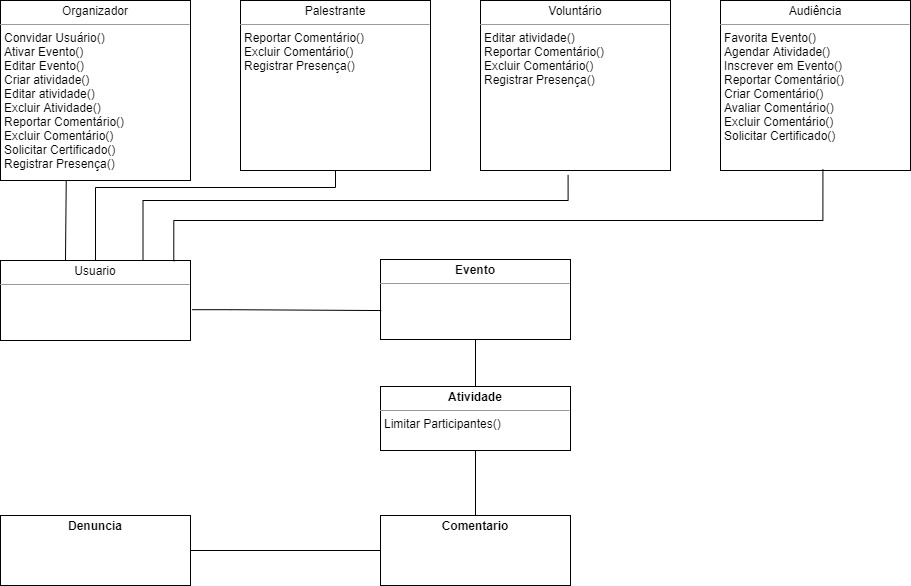
\includegraphics[scale=0.49]{figuras/diagrama-classe-conceitual.jpg}}
    % 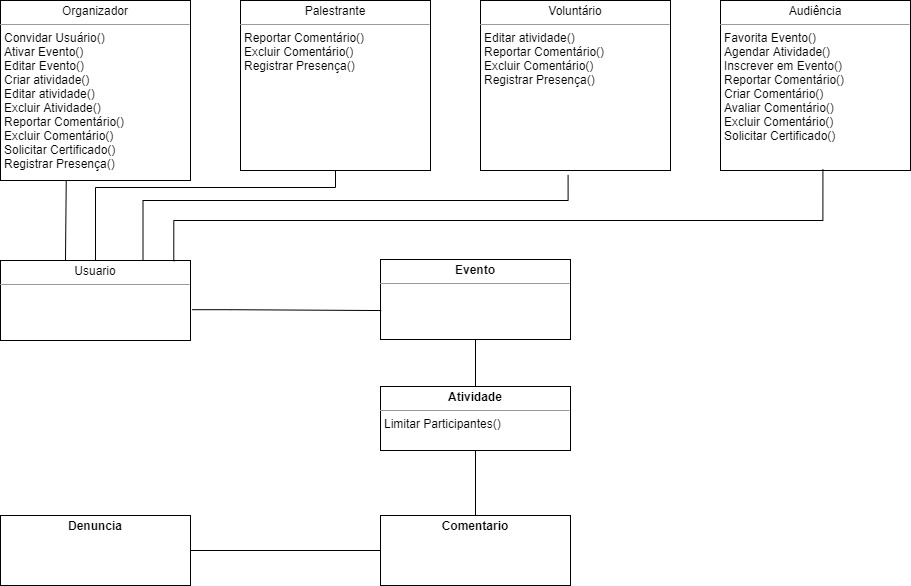
\includegraphics[scale=0.5]{figuras/diagrama-classe-conceitual.jpg}
    \label{fig:digrama-classe}
    \legend{Fonte: elaborado pelos autores}
\end{figure}

\section{Validação e execução em ambiente real}

Em novembro de 2019, no IFF Campos Centro, ocorreu o evento CITI. Ocorreram nesse evento atividades como palestras, minicursos e mesas redondas, atividades as quais necessitavam registro de presença dos participantes para geração dos certificados. Foi observado, pelos organizadores do evento, a necessidade de uma ferramenta para agilizar o registro dessas presenças. 

Diante disso, foi desenvolvido pelos os autores deste trabalho um aplicativo para dispositivos com sistema operacional \textit{Android} para atender a essa necessidade, o qual também foi utilizado para validação e estudo de parte da solução proposta deste trabalho. O aplicativo foi desenvolvido utilizando a \textit{framework} para desenvolvimento híbrido \textit{Ionic}. No entanto, foi utilizado a técnica de \textit{Minimum Viable Product} (MVP), conforme descrito por \citeonline{ries2014lean}. O objetivo foi construir um aplicativo com recursos e funcionalidades mínimas, porém viáveis, para o processo de registro de presença no evento.

Além do aplicativo, foi desenvolvida uma \textit{Application Programming Interface} (API), na linguagem PHP, que foi hospedada no servidor do IFF Campos Centro, onde possuía apenas uma rota, usando o verbo \textit{Hypertext Transfer Protocol} (HTTP) GET, para registrar a presença em um servidor \textit{Structured Query Language} (SQL). Era armazenado os seguintes dados:

\begin{itemize}
    \item CPF do participante;
    \item Nome do participante;
    \item Identificador da atividade o qual está participando;
    \item Data e hora do registro;
    \item Nome do voluntário que está realizando o registro.
\end{itemize}

O registro era feito na entrada e saída da atividade, e a informação da data e hora do registro era usada para calcular posteriormente o tempo em que o participante ficou na atividade, ajudando na validação para a geração do certificado. Além de registrar utilizando a API, também era gerado um registro dessas presenças em um arquivo \textit{Comma-Separated Values} (CSV) no dispositivo do usuário, com a finalidade de haver um \textit{backup} em caso de perdas no banco de dados.

O aplicativo era composto por duas telas. Na primeira tela, haviam dois campos, um de texto para o voluntário informar seu nome, e outro campo para o voluntário selecionar qual atividade vai ser registrada a presença. Abaixo haviam dois botões, um para prosseguir para a tela de leitura de \textit{QRCode} para registrar a presença do participante. O segundo botão abria o leitor de \textit{QRcode} do dispositivo \textit{Android} para registrar a presença de outro voluntário no dia do evento. Na Figura \ref{fig:mvp1} é apresentada esta tela.

\begin{figure}[H]
    \centering
    \caption{Tela inicial do MVP} 
    % 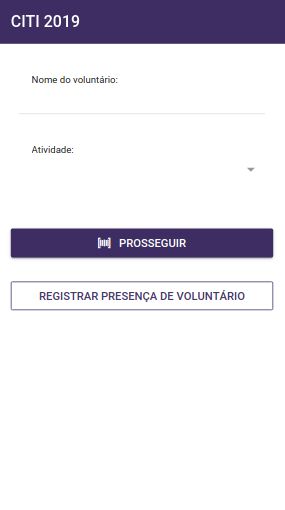
\includegraphics[scale=0.7]{figuras/mvp1.png}
    \fbox{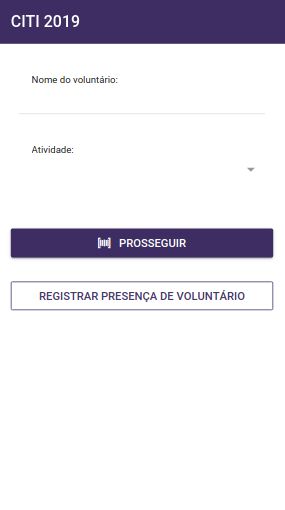
\includegraphics[scale=0.7]{figuras/mvp1.png}}
    \label{fig:mvp1}
    \legend{Fonte: elaborado pelos autores}
\end{figure}

Na segunda tela havia apenas um botão, ao qual abria o leitor de \textit{QRCode} para registrar a presença do participante (Figura \ref{fig:mvp2}). O \textit{QRCode} lido estava nos crachás de identificação dos participantes distribuídos durante o evento. No \textit{QRCode} contido nos crachás, havia a informação do nome do participante e CPF, o qual era capturado pelo aplicativo.

\begin{figure}[H]
    \centering
    \caption{Tela de leitura de \textit{QRCode} de credenciamento do MVP}
    % 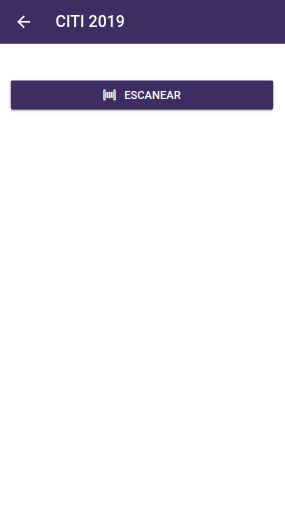
\includegraphics[scale=0.7]{figuras/mvp2.png}
    \fbox{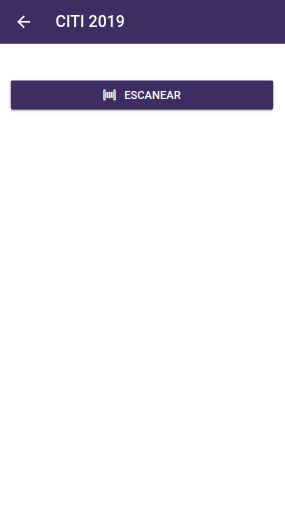
\includegraphics[scale=0.7]{figuras/mvp2.png}}
    \label{fig:mvp2}
    \legend{Fonte: elaborado pelos autores}
\end{figure}

\section{Análise do resultado da execução em ambiente real}

Esse MVP foi utilizado por 12 discentes que formavam parte do comitê organizador do CITI. Ao final do evento, foi produzido e distribuído pelos autores deste trabalho um questionário avaliativo, utilizando a ferramenta \textit{Google Forms}, para esses discentes. Foram obtidas 11 respostas. Esse questionário teve como finalidade saber a opinião dos usuários quanto a usabilidade e solução proposta pelo aplicativo. O questionário possuía as seguintes perguntas:

\begin{itemize}
    \item A tela de credenciamento é intuitiva?
    \item A tela de leitura do \textit{QRCode} é intuitiva?
    \item De modo geral a aplicação foi de fácil utilização?
    \item O arquivo de \textit{backup} local foi de fácil acesso?
    \item Aplicação apresentou algum tipo de falha?
    \item Caso apresentou falha, descreva.
    \item Sugestões de melhorias.
\end{itemize}

Com as respostas obtidas pelo formulário, foi observado que o \textit{layout} das telas foram bem aceito, com 100\% das respostas indicando que eram intuitivas e de fácil utilização. Não foi indicado nenhuma falha na utilização do aplicativo. Como sugestões, foi informado uma melhoria na funcionalidade de \textit{backup} e colocar mais imagens no aplicativo. O formulário utilizado para a pesquisa de opinião está disponível no Apêndice \ref{apendice1}, assim como o resultado obtido pelo formulário, onde se encontra no Apêndice \ref{apendice2}.

\section{Desenho da estrutura e funcionalidades}

Após análise dos resultados obtidos com a utilização do aplicativo para credenciamento no CITI, foi iniciado a análise da plataforma Eventos IFF, onde foi avaliado as suas funcionalidades e quais funcionalidades poderiam ser acrescentadas com uma aplicação móvel, baseado na experiência obtida no CITI. Foram feitos levantamentos de requisitos para entendimento melhor da plataforma. 

Ao finalizar essa etapa, foi desenhado \textit{wireframes} ilustrando as funcionalidades vistas inicialmente como relevantes para o aplicativo. Na Figura \ref{fig:wireframe1} e \ref{fig:wireframe2} é mostrado dois \textit{wireframes} desenvolvidos nessa etapa, o primeiro ilustrando a página principal do aplicativo e o segundo com a primeira estrutura idealizada para a funcionalidade de envio de perguntas para o palestrante.

% \begin{figure}[H]
%   \begin{minipage}[b]{0.4\textwidth}
%     \caption{Wireframe da tela inicial do aplicativo}
%     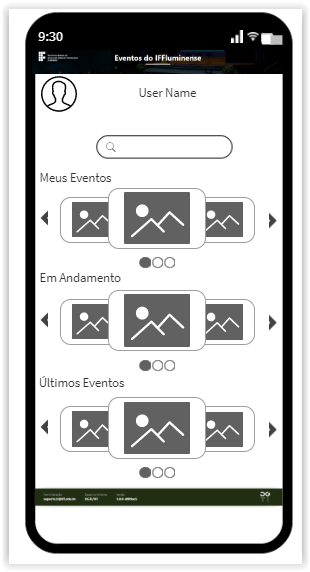
\includegraphics[width=\textwidth]{figuras/wireframe1.PNG}
%     \label{fig:wireframe1}
%     \legend{Fonte: elaborado pelos autores}
%   \end{minipage}
%   \hfill
%   \begin{minipage}[b]{0.4\textwidth}
%     \caption{Wireframe da tela de envio de comentários em atividade}
%     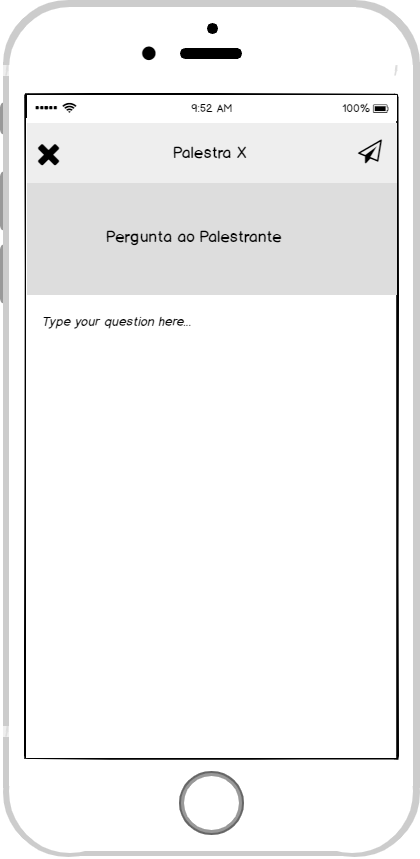
\includegraphics[scale=0.37]{figuras/wireframe2.png}
%     \label{fig:wireframe2}
%     \legend{Fonte: elaborado pelos autores}
%   \end{minipage}
% \end{figure}

\begin{figure}[H]
    \centering
    \caption{\textit{Wireframe} da tela inicial do aplicativo}
    % 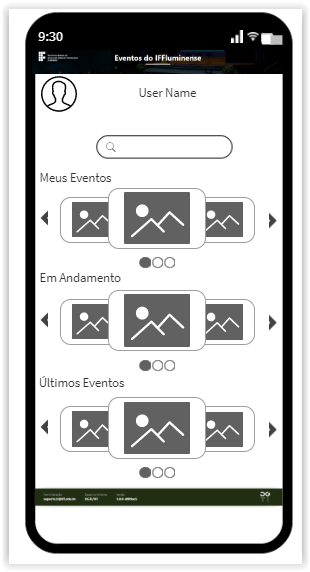
\includegraphics[scale=0.81]{figuras/wireframe1.PNG}
    \fbox{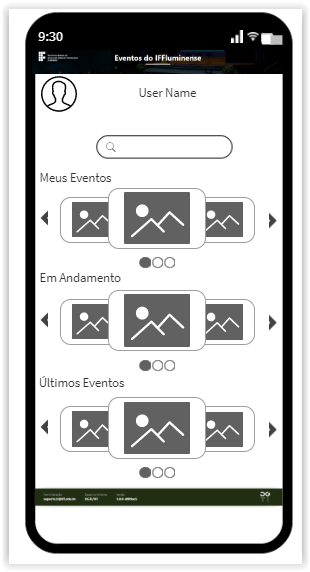
\includegraphics[scale=0.81]{figuras/wireframe1.PNG}}
    \label{fig:wireframe1}
    \legend{Fonte: elaborado pelos autores}
\end{figure}

\begin{figure}[H]
    \centering
    \caption{\textit{Wireframe} da tela de envio de comentários em atividade}
    % 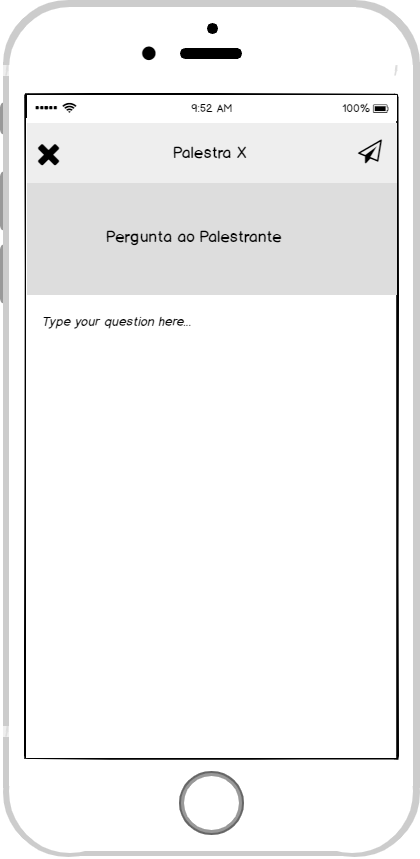
\includegraphics[scale=0.4]{figuras/wireframe2.png}
    \fbox{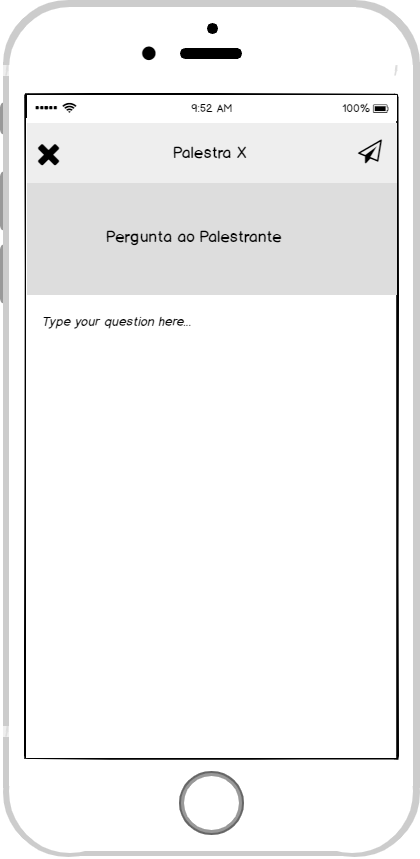
\includegraphics[scale=0.4]{figuras/wireframe2.png}}
    \label{fig:wireframe2}
    \legend{Fonte: elaborado pelos autores}
\end{figure}

Com a definição das funcionalidades e requisitos, foram desenvolvidos os diagramas de caso de uso e de classe. Com esses diagramas, alguns impedimentos e correções nas funcionalidades inicialmente pensadas ficaram mais esclarecidas, o que foram corrigidas com novas revisões nos requisitos levantados e correções nos diagramas. Em seguida foi desenhada a arquitetura dessa solução, visando ilustrar como seria a comunicação entre os serviços do Eventos IFF com o \textit{website} Eventos IFF e o aplicativo proposto por esse trabalho, além da comunicação com a plataforma \textit{Firebase}.

Nas Figuras \ref{fig:classe} é apresentado o diagrama de classe da aplicação. Na Figura \ref{fig:arquitetura} é ilustrada a arquitetura da integração do aplicativo com os serviços do Eventos IFF, assim como com o \textit{Firebase}.

\begin{figure}[H]
    \centering
    \caption{Diagrama de classe}
    % 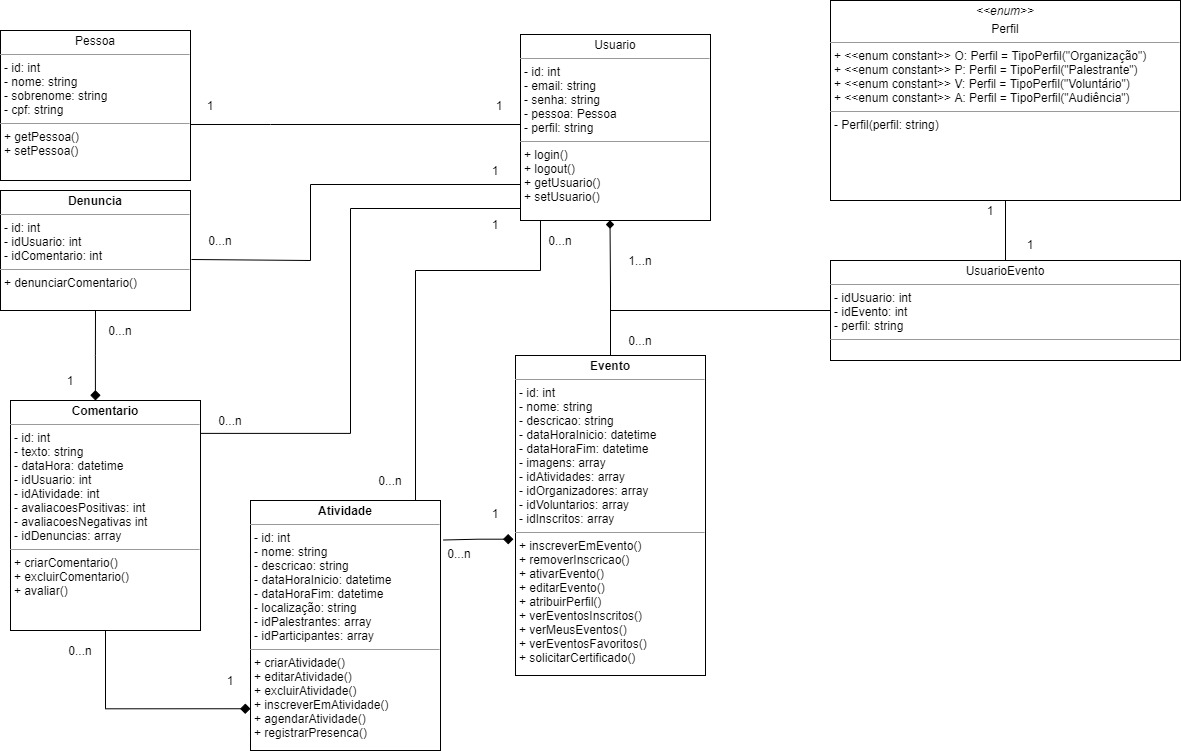
\includegraphics[scale=0.4]{figuras/Diagrama-de-classe.jpg}
    \fbox{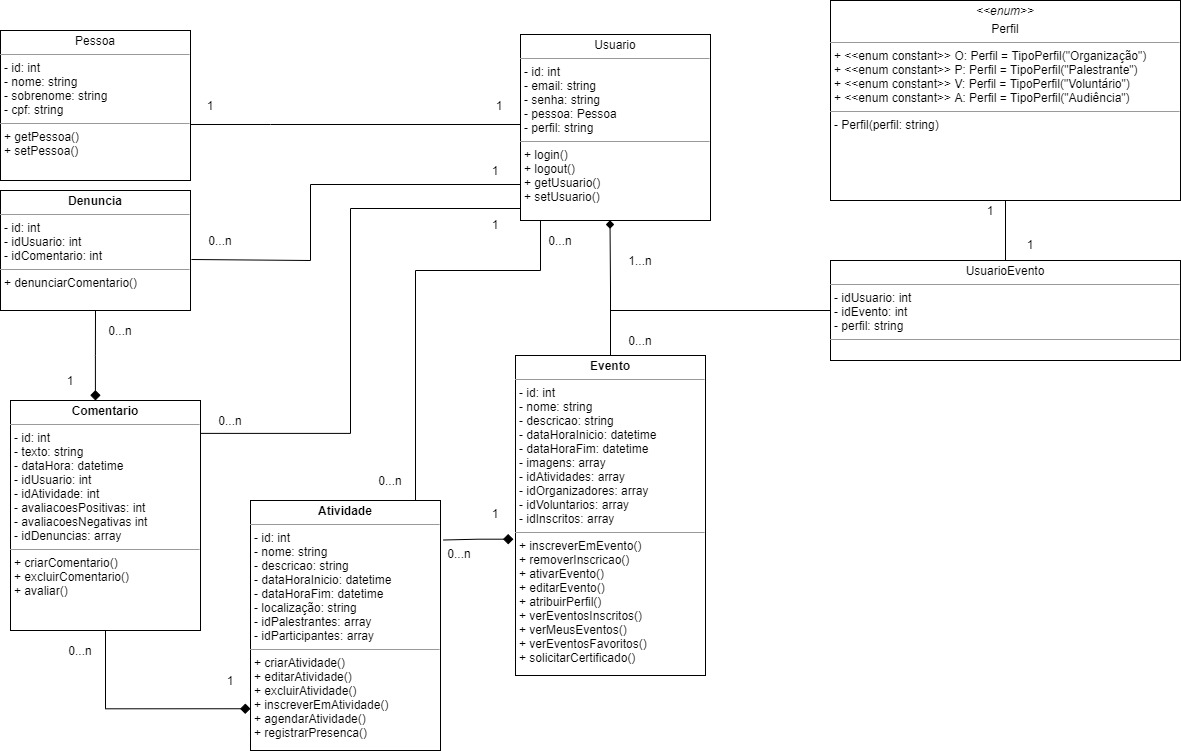
\includegraphics[scale=0.365]{figuras/Diagrama-de-classe.jpg}}
    \label{fig:classe}
    \legend{Fonte: elaborado pelos autores}
\end{figure}

\begin{figure}[H]
    \centering
    \caption{Arquitetura da integração do aplicativo com o Eventos IFF}
    % 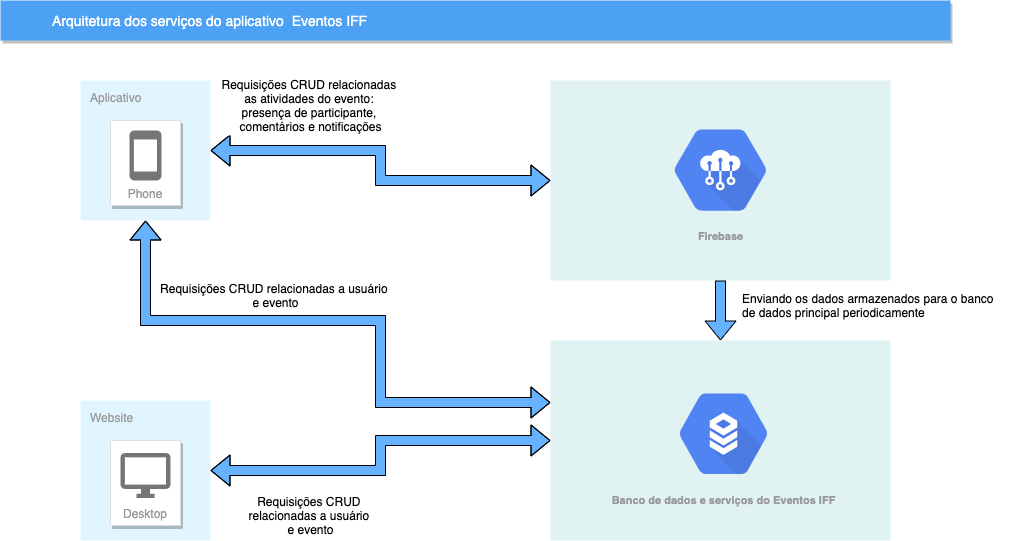
\includegraphics[scale=0.475]{figuras/Arquitetura.png}
    \fbox{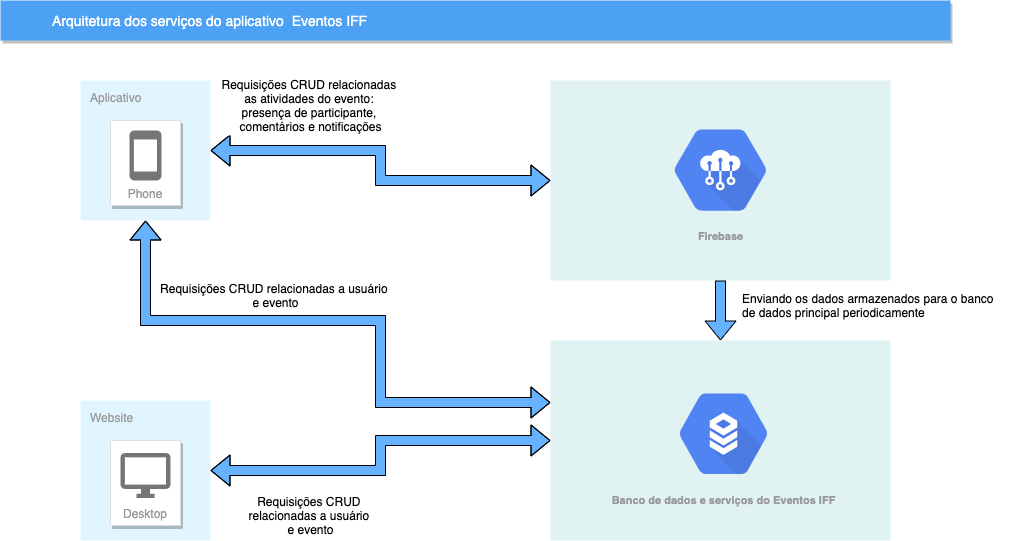
\includegraphics[scale=0.445]{figuras/Arquitetura.png}}
    \label{fig:arquitetura}
    \legend{Fonte: elaborado pelos autores}
\end{figure}

\subsection{Uso do \textit{Firebase} na arquitetura}

O \textit{Firebase} possui uma ferramenta, no qual é chamada de \textit{Firestore Database} ou \textit{Cloud Firestore}, onde consiste em um banco de dados não relacional, flexível e escalonável, que é indicado para desenvolvimento de dispositivos móveis, além de aplicações \textit{web} \cite{google_firebase}.

O \textit{Firestore Database} oferece uma sincronia em tempo real entre o dispositivo cliente e o banco de dados. Isso é possível através de ouvintes que atuam no dispositivo cliente através da integração com o \textit{Firestore Database}, onde atualiza os dados no dispositivo cliente logo após sua mudança no banco de dados \cite{google_firebase}. Na Figura \ref{fig:firebase} é exibido um exemplo da estrutura de armazenamento do \textit{Firestore Database} na interface do \textit{Firebase}.

\begin{figure}[H]
    \centering
    \caption{Interface do \textit{Firestore Database} no \textit{Firebase}}
    % 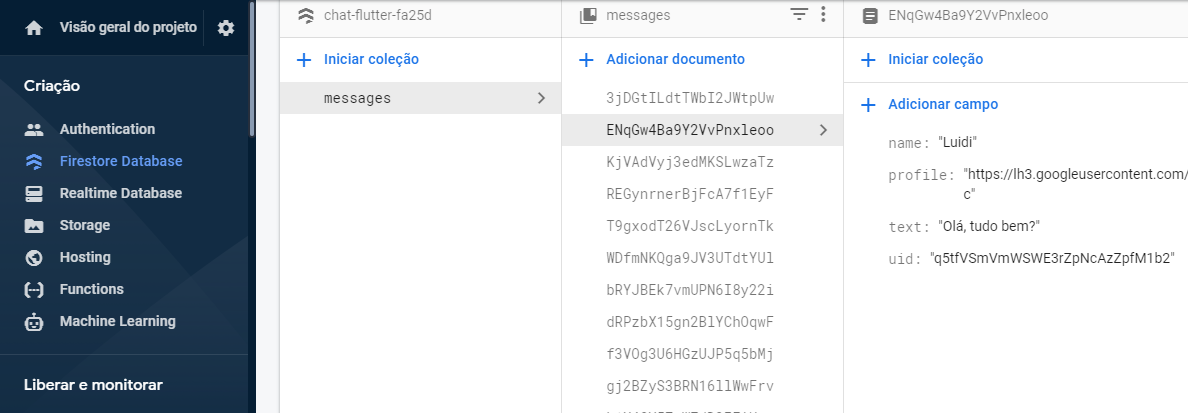
\includegraphics[scale=0.5]{figuras/firebase.PNG}
    \fbox{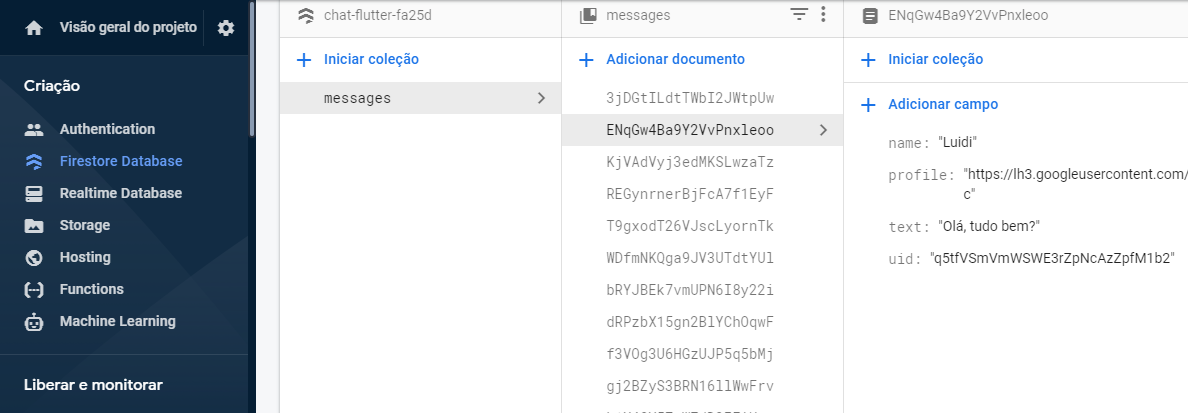
\includegraphics[scale=0.503]{figuras/firebase.PNG}}
    \label{fig:firebase}
    \legend{Fonte: \textit{website} do \textit{Firebase}}
\end{figure}

Deste modo, para a funcionalidade de comentários na atividade do aplicativo Eventos IFF, essa sincronia em tempo real do \textit{Firestore Database} se torna fundamental para uma boa experiência do usuário, onde os novos comentários feitos por outros usuários na atividade são exibidos em tempo real para o usuário que estiver visualizando essa tela.
\chapter{Conclusão}

No processo de desenvolvimento deste trabalho foram seguidas as etapas de análise, estudo e levantamento de requisitos, que são fundamentais para o desenho e desenvolvimento de \textit{softwares}.

Com a execução da técnica de MVP em um evento acadêmico real, foi observado as reais necessidades para esse cenário, e utilizando a pesquisa de opinião da utilização desse MVP possibilitou um melhor esclarecimento da solução desejada.

Deste modo, foi possível realizar os levantamentos com um especialista da plataforma IFF Eventos, e o mesmo considerou satisfatório os resultados obtidos. A partir disso foi constatada a viabilidade do desenvolvimento de uma solução para uma ferramenta que agregasse funcionalidade e agilidade no gerenciamento de eventos da plataforma.

O desenho de diagramas de uso, diagrama de classe conceitual e diagramas de arquitetura foram fundamentais para prosseguir com o desenvolvimento do protótipo de forma mais segura e assertiva, visto que esses diagramas possibilitam um entendimento mais claro do \textit{software} e seu contexto, evitando futuros imprevistos no desenvolvimento.

Paralelamente, foi visto que a técnica de prototipagem auxilia no processo de desenvolvimento de \textit{software}. A construção de um protótipo interativo coopera na visualização da solução, trazendo assim mais facilidade para o desenvolvimento das telas do \textit{software}, uma vez que a etapa visual já está desenhada. 

Por fim, a partir desse desenho de solução, experimentado a partir deste protótipo, foi possível direcionar o sistema, melhorando assim os processos de gerenciamento, bem como otimizando a experiência da audiência nos eventos.



% ----------------------------------------------------------
% ELEMENTOS PÓS-TEXTUAIS
% ----------------------------------------------------------
\postextual
% ----------------------------------------------------------

% ----------------------------------------------------------
% Referências bibliográficas
% ----------------------------------------------------------
\bibliography{referencias.bib}


%---------------------------------------------------------------------
% INDICE REMISSIVO
%---------------------------------------------------------------------
\phantompart
\printindex
%---------------------------------------------------------------------

\end{document}
